\documentclass{article}
\usepackage[utf8]{inputenc}
\usepackage{amsmath}
\usepackage{mathtools}
\usepackage[a4paper,left=0.8in,right=0.8in,bottom=1in]{geometry}
\setlength{\parskip}{1em}
\setlength{\parindent}{0em}
\usepackage{floatrow}
\usepackage{graphicx}
\renewcommand{\familydefault}{\ttdefault}
\title{\huge\texttt{CS215 Assignment 4}}
\author{Aquib Nawaz(190050023),Rajesh Dasari(190050030),\\\texttt{Paavan Kumar(190050051)}}
\date{\texttt{11 November 2020}}

\begin{document}

\maketitle

\section* {Question 1}
\subsection* {a)}
$X_1$,$X_2$ are uniformly distributed ,\\hence $P(X_1=a) = \frac{1}{2}$ for $-1<a<1$ and $P(X_2=b) = \frac{1}{2}$ for $-1<b<1$.
\\
Therefore , we have $P(X = (a,b)) = P(X_1=a,X_2=b)$\\
$P(X=(a,b)) = P(X_1=a)P(X_2=b) = \frac{1}{4}$
\\
Now to calculate the probability that the point lies in a circle of radius 1 , we integrate the probability $p_X(a,b)$ over the area of the circle.\\ let the area of circle be A\par
Hence, $p = \int\int_{x,y \in A} p_X(x,y) dx dy$\\
$p = \int\int_{x,y \in A} \frac{1}{4} dx dy$\\
$p = \frac{1}{4} \int\int_{x,y \in A} dx dy$\\
$p = \frac{1}{4}A$\\
Therefore  $\boxed{p = \frac{\pi}{4}}$
\subsection*{b)}
Suppose N is the sample size of the random variable generated for computing the value of $\pi$.\\
And Y be the number of points that actually lie inside the circle when we plot the values of $X=(X_1,X_2)$ taking $X_1$ on the x-axis and $X_2$ on y-axis\\
Then by the formula determined above $p = \frac{\pi}{4}$\\
We also know  that actual probability $p = \frac{Y}{N}$ \\
Hence equating both we get the value of $\pi$  to be $\frac{4Y}{N}$
\subsection*{c)}
The code for this part is attached with the name $q1.m$ in the Code folder\\
Our code doesnt handle this case, since we generate a N smaple and the count the values that lie in the region bounded by the circle\\
Generating a random sample of size $10^9$ usually takes a lot of time in MATLAB, so this is not a very good idea , so instead we can use the bernoullli confidence interval and estimate the value of $\pi$ using the formula mentioned in part D
\begin{equation}
    \hat{p} \pm z\sqrt{\frac{(1-\hat{p})\hat{p}}{M}}
\end{equation}
Given the value of M which is the sample size , we can calculate the value of z and hence estimate the confidence interval and we can cut the value of $\pi$ estimated to a small range with more than $99\%$ confidence interval\\
\subsection*{d)}
Lets take each trail to be a Bernoulli trial with parameter $p = \pi/4$, Here if the the chosen point in a trial lies in the circle then it will be considered success else failure.\\
Now we know for a binomial distribution $p$ is estimated as 
\begin{equation}
    \hat{p} \pm z\sqrt{\frac{(1-\hat{p})\hat{p}}{M}}
\end{equation}
Where $z$ for $95\%$ confidence interval is 1.96 and $M$ is size of data points.\\
Also error in $\pi$ is $4\times$ error in $\hat{p}$
We can find $M$ from here which turns out to be around $100000$ using $\pi = 3.141592$ and $\hat{p}=\pi/4$.
\section*{Question 2}
\subsection*{a)}
A general multivariate gaussian variable is given by $X = AW + \mu$ \\
Its coefficient matrix $C = A A^T$. So to generate random sample of given distribution we have to first find A.\\
Now covariance $C$ is a symmetric positive definite matrix so it can be written as $QDQ^T$.\\ Where $Q$ is an orthogonal matrix whose columns are the eigenvectors of $C$, and $D$ is a diagonal matrix whose entries are the eigenvalues of $C$.\\
Hence $C = QDQ^T = (Q\sqrt{D})(\sqrt{D}Q^T) = (Q\sqrt{D})(Q\sqrt{D})^T$ as entries in $D$ are positive.\\
Hence one possible value of $A$ is $Q\sqrt{D}$.\\
$Q$ and $D$ can be obtained by eig() function and $W$ can be obtained by randn() function. 

The code for this question is attached as $q2.m$

\section*{Question 3}
\subsection*{a)}
Principal component analysis can be used to find a linear fit for scatter plots\\
First we determine the mean of the two varaibles X,Y (name it as $m_1,m_2$)\\
By PCA, the linear fit must pass through the $(m_1,m_2)$\\
Now we determine the variance and co-variance of the random variables X,Y (name them $v_1,v_2, c$\\
Now we transform the X,Y to X-$m_1$,Y-$m_2$(actually this is not necessary)\\
Then assume a unit vector $v$,$[\cos(\theta),\sin(\theta)]'$ along the direction of the resultant linear fit,\\$slope = \tan(\theta)$\\
Now by PCA , we have to maximise the value of $v'Cv$ where $v'$ is the transpose of vector $v$\\
Here C is the covariance matrix $[[v_1 c][c v_2]]$\\
Hence expanding $v'Cv$ we get an expression E\par 
$E = v_1\cos(\theta)^2+v_2\sin(\theta)^2+2c\cos(\theta)\sin(\theta)$\\
Differentiating w.r.t $\theta$, we get \par 
$(v_2-v_1)\sin(2\theta) + 2c \cos(2\theta)) = 0 \implies \tan(2\theta) = \frac{2c}{v_1-v_2}$ and Hence $\boxed{\theta = \frac{1}{2}\arctan{\frac{2c}{v_1-v_2}}}$
\subsection*{b)}
The code for this part is attached with the name $q3b.m$ \\
The scatter plot overlaid with plot for pca is attached below\\
\ffigbox{\caption {points2D Set1}}
    {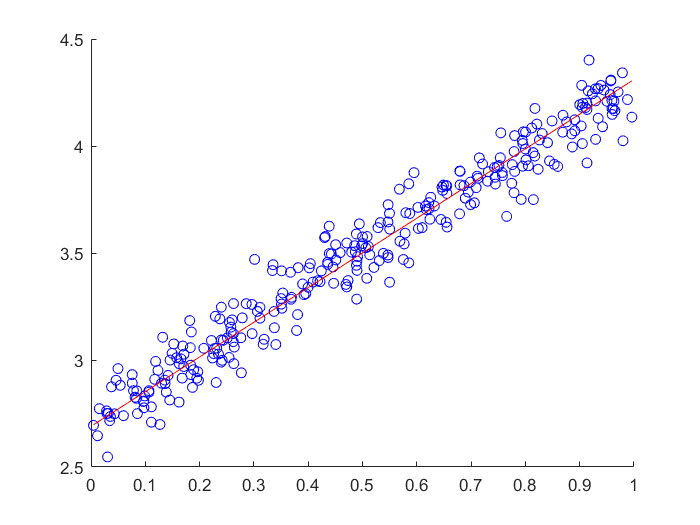
\includegraphics[width =10cm, height=8cm]{hw4/q3b.png}}
\subsection*{c)}
The code for this part is attached with the name $q3c.m$ \\
The scatter plot overlaid with plot for pca is attached below\\
Since the covariance of the set of vaues of X and Y is approximately 0,the value of theta\\ determined from the relation in part a) comes out to be zero, this is a pretty bad approximation of the graph since we are assuming the graph to be linear where in practical its not zero , for example the set 2 given has approx zero correlation and hence the outcome of the result is quite unsuitable.\\
\ffigbox{\caption {points2D Set2}}
    {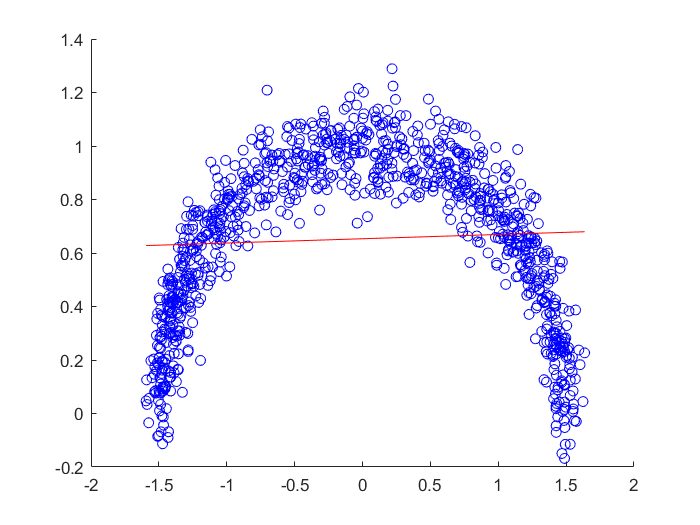
\includegraphics[width =10cm, height=8cm]{hw4/q3c.png}}\\
The quality of approximation use for this part is very poor since we actually don't know that the data is scattered around a line , which is the assumption that we made in the pca part to estimate the direction of maximal variance, But from the scatter plot we can actually say that the data is distributed along a semicircular arc,and only one dimension is enough to find the direction of maximal variance it may be a curved direction depending on the distance from origin\\ 
\section*{Question 4}
MATLAB code for this question is attached as Q4.m

On plotting eigen values for different digits we found that the number of significant eigen values is around 100 which is far less than 784.\\ 
It means that value of only few pixels varies much among all the images of same digit.\\ It is because some style or orientation of digit may change but its basic skeleton remain same.

On plotting three images for each digit we found that the mode of variation showing images  are tilted around its mean. So people deviates in writing. 

For digit 1 in third image it is tilted more rightward while first image is straight which means some people write it mostly straight while other more toward tilted write.

\section*{Question 5}
Code for this question is attached as q5.m\\
The code written by us for this part is slightly slower than usual time\\
\section*{Question 6}
Code for this Question is attached as q6.m
\subsection*{a)}
The plot for mean and first four eigen vectors have been attached in the $results$ folder\\
\ffigbox{\caption {first 10 eigen values}}
    {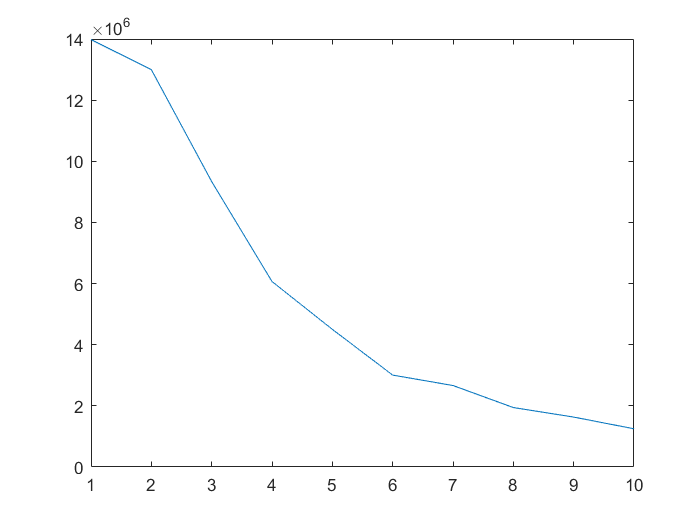
\includegraphics[width =10cm, height=8cm]{hw4/q6_eigenvalues.png}}\\
\subsection*{b)}
Let $sz = size(I)$
Let the eigen vectors be $\Vec{V_1},\Vec{V_2},\Vec{V_3},\Vec{V_4}$ found out from the first part. \\let $I'$ be the closest representation of the image $I$ in terms of the mean $\Vec{\mu}$ and the eigen vectors\par
$I' = a_0\Vec{\mu} + \sum_1^4 a_i\Vec{V_i}$                         \par 
Our job is to minimise $I-I'$\\
Therefore to minimise  the magnitude of $T = I-I'$\par 
Let $T[j] = I[j] - a_0\Vec{\mu}[j] - \sum_0^4 a_i \Vec{V_i}[j] $\par 
Therefore to minimise the value of $F(a_0,a_1,a_2,a_3,a_4) = \sum_1^{sz} T[j]\times T[j]$\par 
Differentaiting w.r.t $a_i,i\neq0$, we get\par 
$\frac{\partial F}{\partial a_i} = \sum_1^{sz} 2\times T[j] \times \frac{\partial T[j]}{\partial a_i} $\par
We Know for $i\neq 0$,$\frac{\partial T[j]}{\partial a_i} = -\Vec{V_i}[j]$\par 
Therefore ,$\frac{\partial F}{\partial a_i} = \sum_1^{sz} 2\times T[j] \times -\Vec{V_i}[j] $\par 
Hence $\frac{\partial F}{2\partial a_i} = -I\cdot\Vec{V_i}+a_0 \Vec{V_i}\cdot\Vec{\mu} + \sum_{j=1}^4 a_j\Vec{V_i}\cdot\Vec{V_j} = -I\cdot\Vec{V_i}+a_0 \Vec{V_i}\cdot\Vec{\mu} + a_i\Vec{V_i}\cdot\Vec{V_i}+\sum_{j\neq i} a_j\Vec{V_i}\cdot\Vec{V_j}$\par 
Since these are eigen vectors of a covariance matrix, $\Vec{V_i}\cdot\Vec{V_j}=0$ for $j\neq i$ and $\Vec{V_i}\cdot\Vec{V_i} = 1$\par 
Therefore, $\frac{\partial F}{2\partial a_i} = -I\cdot\Vec{V_i}+a_0 \Vec{V_i}\cdot\Vec{\mu}+a_i $\par 
Equating to zero , we get $\frac{\partial F}{2\partial a_i} = -I\cdot\Vec{V_i}+a_0 \Vec{V_i}\cdot\Vec{\mu}+a_i = 0 \implies \boxed{a_i = I\cdot\Vec{V_i}-a_0 \Vec{V_i}\cdot\Vec{\mu}\ \ \ \  \ ,i\neq 0} $\par 
Now similarly differentiating w.r.t $a_0$, we get \par 
$\frac{\partial F}{\partial a_0} = \sum_1^{sz} 2\times T[j] \times \frac{\partial T[j]}{\partial a_0} $\par
We Know for $\frac{\partial T[j]}{\partial a_0} = -\Vec{\mu}[j]$\par 
Therefore ,$\frac{\partial F}{\partial a_i} = \sum_1^{sz} 2\times T[j] \times -\Vec{\mu}[j] $\par
Hence, $\frac{\partial F}{2\partial a_0} = -I\cdot\Vec{\mu}+a_0 \Vec{\mu}\cdot\Vec{\mu} + \sum_{i=1}^4 a_i\Vec{\mu}\cdot\Vec{V_i} = -I\cdot\Vec{\mu}+a_0 \Vec{\mu}\cdot\Vec{\mu} + \sum_{i=1}^4 (I\cdot\Vec{V_i}-a_0 \Vec{V_i}\cdot\Vec{\mu})\Vec{\mu}\cdot\Vec{V_i} $\par 
Therefore, $\frac{\partial F}{2\partial a_0} = a_0(\Vec{\mu}\cdot\Vec{\mu}-\sum_{i=1}^4 {(\Vec{\mu}\cdot\Vec{V_i})}^2) - (I\cdot\Vec{\mu} - \sum_{i=1}^4 ((I\cdot\Vec{V_i})(\Vec{\mu}\cdot\Vec{V_i}) )$\par 
Equating to zero, we get $\boxed{a_0 = \frac{I\cdot\Vec{\mu} - \sum_{i=1}^4 (I\cdot\Vec{V_i})(\Vec{\mu}\cdot\Vec{V_i})}{\Vec{\mu}\cdot\Vec{\mu}-\sum_{i=1}^4 {(\Vec{\mu}\cdot\Vec{V_i})}^2}}$\par 
And Therefore, $a_i =I\cdot\Vec{V_i} - \frac{I\cdot\Vec{\mu} - \sum (I\cdot\Vec{V_i})(\Vec{\mu}\cdot\Vec{V_i})}{\Vec{\mu}\cdot\Vec{\mu}-\sum {(\Vec{\mu}\cdot\Vec{V_i})}^2} \Vec{V_i}\cdot\Vec{\mu} , i\neq 0  $ and $a_0 = \frac{I\cdot\Vec{\mu} - \sum_{i=1}^4 (I\cdot\Vec{V_i})(\Vec{\mu}\cdot\Vec{V_i})}{\Vec{\mu}\cdot\Vec{\mu}-\sum_{i=1}^4 {(\Vec{\mu}\cdot\Vec{V_i})}^2}$\par 
The plots thus obtained are placed in the $results$ folder with the name $q\_i.png$ where each image corresponds to the ith fruit.\\
One such image is below as for image 16 where the fruit is an apple\\
\ffigbox{\caption {original and closest}}
    {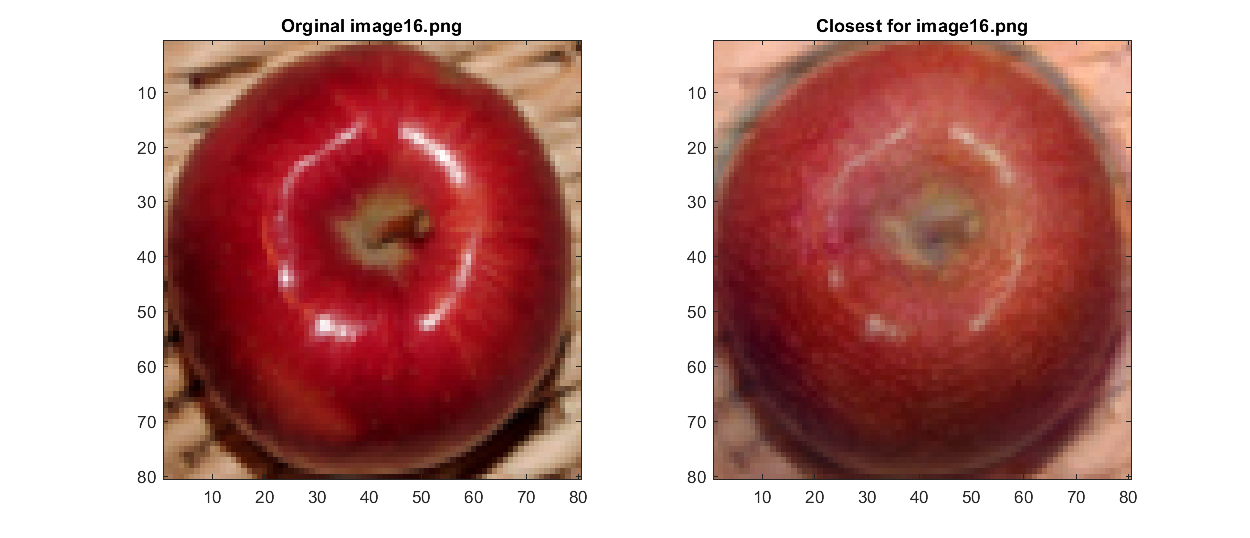
\includegraphics[width =16cm, height=7cm]{hw4/q6_16.png}}\\
This can be done in another way by considering the co-efficient of mean to be 1 and fitting the data onto the first four eigen vectors, called 4-D hyperplane fitting, we find the co-eff in the same as found out above the mean co-eff would be 1 which means $\boxed{a_i = (I-\Vec{\mu})\cdot\Vec{V_i}\ \ \ \  \ ,i\neq 0}$, from this we can find out the closest representation in the 4D hyperplae formed by the four eigen vectors
\subsection*{c)}
Let The eigen values corresponding to those four eigen vectors placed along a diagonal of a 4 by 4 matrix, name this matrix $D$ can be computed using eigs function eficiently\\
With matrix as diagonal eigen valued matrix , we can find the matrix A for standard normal\\ distribution given the eigen valued matrix as follows\\
$A = V'\sqrt{D}V$ \\
Now we generate a random sample of size 19200,and using the relation X = AW + $\mu$, we get a new fruit value with th egiven mean and eigen vectors as $V$
W is a gaussian random variable that can be generated by using randn(19200,1) in matlab

\end{document}